% =====================================================================
\section{Experimental Programme}
\label{sec:experiments}
% =====================================================================

The model of Section~\ref{sec:model} is implemented as a JAX-vectorised
extension of pymdp. Four experiments are designed to characterise the
joint role of cost of mind-change $\stub$ and channel precision
$\trust{i}{j}$ in the population dynamics. We summarise the design
here and defer the empirical figures.

\paragraph{E1 (Baseline).}
Stationary environment, $\stub = 0$ for all agents. Sanity check on
the implementation: under the limit of Proposition~\ref{prop:limit},
$\C_V^{(t)}$ should track $\hidden^{*}$ tightly with no
systematic lag.

\paragraph{E2 (Adaptation lag under shock).}
Discrete-shift environment with deterministic flip of one feature at
$t = t^{*}$. Sweep $\stub$. The expected observable is monotonic
adaptation lag $\tau(\stub)$: low-$\stub$ communities recover within a
few timesteps, high-$\stub$ communities persist in the pre-shift
salience landscape well past $t^{*}$.

\paragraph{E3 (Hysteresis under slow drift).}
Slow-drift environment in which $\hidden^{*}$ traces a forward
trajectory $A \to B$ followed by a reverse trajectory $B \to A$. Sweep
$\stub$. The headline figure is the family of hysteresis loops in
$(\hidden^{*}, \C_V)$ space; loop area $\propto \stub$
(Proposition~\ref{prop:limit}). Figure~\ref{fig:hysteresis-schematic}
shows the predicted loop shape.

\begin{figure}[t]
\centering
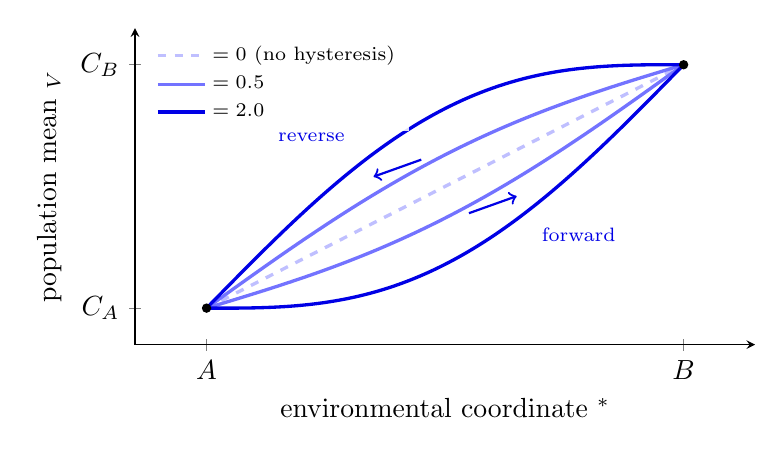
\begin{tikzpicture}
\begin{axis}[
  width=0.78\linewidth, height=5.6cm,
  xlabel={environmental coordinate $\hidden^{*}$},
  ylabel={population mean $\C_V$},
  xmin=-0.15, xmax=1.15,
  ymin=-0.15, ymax=1.15,
  xtick={0,1}, xticklabels={$A$, $B$},
  ytick={0,1}, yticklabels={$C_A$, $C_B$},
  axis lines=left,
  legend style={font=\scriptsize, draw=none,
                at={(0.02,0.98)}, anchor=north west,
                fill=white, fill opacity=0.85, text opacity=1},
  legend cell align=left,
  every axis plot/.append style={very thick}
]
% lambda = 0: identity line, no loop
\addplot[domain=0:1, samples=40, color=blue!25, dashed]
  {x};
\addlegendentry{$\stub = 0$ (no hysteresis)}

% lambda = 0.5: small loop
\addplot[domain=0:1, samples=80, color=blue!55,
         smooth]
  ({x}, {x - 0.13*sin(deg(pi*x))});
\addlegendentry{$\stub = 0.5$}
\addplot[domain=0:1, samples=80, color=blue!55,
         smooth, forget plot]
  ({1-x}, {(1-x) + 0.13*sin(deg(pi*(1-x)))});

% lambda = 2.0: large loop
\addplot[domain=0:1, samples=80, color=blue!90!black,
         smooth]
  ({x}, {x - 0.32*sin(deg(pi*x))});
\addlegendentry{$\stub = 2.0$}
\addplot[domain=0:1, samples=80, color=blue!90!black,
         smooth, forget plot]
  ({1-x}, {(1-x) + 0.32*sin(deg(pi*(1-x)))});

% Annotate loop direction with arrows
\draw[->, thick, blue!90!black] (axis cs:0.55, 0.39) -- (axis cs:0.65, 0.46);
\draw[->, thick, blue!90!black] (axis cs:0.45, 0.61) -- (axis cs:0.35, 0.54);
\node[font=\scriptsize, blue!90!black] at (axis cs:0.78, 0.30) {forward};
\node[font=\scriptsize, blue!90!black] at (axis cs:0.22, 0.70) {reverse};

% Mark fixed points
\node[circle, fill=black, inner sep=1.2pt] at (axis cs:0,0) {};
\node[circle, fill=black, inner sep=1.2pt] at (axis cs:1,1) {};

\end{axis}
\end{tikzpicture}
\caption{Predicted hysteresis loops in
$(\hidden^{*}, \C_V)$ space under the slow-drift regime of E3
(schematic, illustrative $\stub$ values). The forward trajectory
$A \to B$ lags the environmental shift; the reverse trajectory
$B \to A$ lags it in the opposite direction. The two trajectories
enclose an area monotone in $\stub$. The $\stub = 0$ limit
(Proposition~\ref{prop:limit}) collapses the loop to the identity
line.}
\label{fig:hysteresis-schematic}
\end{figure}

\paragraph{E4 (Dissociation from rule-induction).}
Identical environment sequence run on (a) the present model and
(b) a Bayesian rule-induction baseline derived from
\citet{oldenburgZhiXuan2024BayesianRule}. The expected observable is
side-by-side trajectories: symmetric tracking in (b), hysteretic loops
in (a) for any $\stub > 0$.

Each configuration is run for $\geq 20$ random seeds with population
$\Nagents = 30$ on Watts--Strogatz graphs ($k = 6$, $\beta = 0.1$);
reported quantities are mean $\pm 95\%$ confidence intervals.
